\documentclass[a4paper,12pt]{report}

\usepackage{fullpage}
\usepackage{url}
\usepackage{makeidx}
\usepackage{verbatim}
\usepackage{graphicx}
\input{./version.tex}

\newcommand{\caml}{\textsf{Caml}}
\newcommand{\pvs}{\textsf{PVS}\index{PVS@\textsf{PVS}}}
\newcommand{\coq}{\textsf{Coq}\index{Coq@\textsf{Coq}}}
\newcommand{\harvey}{\textsf{haRVey}\index{haRVey@\textsf{haRVey}}}
\newcommand{\simplify}{\textsf{Simplify}\index{Simplify@\textsf{Simplify}}}
\newcommand{\mizar}{\textsf{Mizar}\index{Mizar@\textsf{Mizar}}}
\newcommand{\hollight}{\textsf{HOL Light}\index{HOL Light@\textsf{HOL Light}}}
\newcommand{\isabelle}{\textsf{Isabelle/HOL}\index{Isabelle/HOL@\textsf{Isabelle/HOL}}}
\newcommand{\holfour}{\textsf{HOL 4}\index{HOL 4@\textsf{HOL 4}}}
\newcommand{\cvclite}{\textsf{CVC Lite}\index{CVC Lite@\textsf{CVC Lite}}}
\newcommand{\zenon}{\textsf{Zenon}\index{Zenon@\textsf{Zenon}}}
\newcommand{\krakatoa}{\textsf{Krakatoa}\index{Krakatoa@\textsf{Krakatoa}}}
\newcommand{\caduceus}{\textsf{Caduceus}\index{Caduceus@\textsf{Caduceus}}}
\newcommand{\java}{\textsc{Java}\index{Java@\textsf{Java}}}
\newcommand{\jml}{\textsc{JML}\index{JML@\textsf{JML}}}
\newcommand{\why}{\textsf{Why}}
\newcommand{\te}[1]{\texttt{#1}}
\newcommand{\nt}[1]{$\langle$\textsl{#1}$\rangle$}
\newcommand{\indexnt}[1]{\index{#1@\textsl{#1}, grammar entry}}
\newcommand{\indextt}[1]{\index{#1@\texttt{#1}}}
\newcommand{\etoile}{$^{\star}$}
\newcommand{\etoilesep}[1]{$^{\star}_#1$}
\newcommand{\plus}{$^+$}
\newcommand{\plussep}[1]{$^+_#1$}
\newcommand{\caveat}{\paragraph{Caveat.}}
\newcommand{\caveats}{\paragraph{Caveats.}}

\makeindex

\begin{document}

%%% coverpage
\thispagestyle{empty}
\begin{center}
~\\[3cm]
\rule\textwidth{0.1cm}\\[0.5cm]
{\Huge\sf The WHY verification tool}\\[1cm]
{\Large\sf Tutorial and Reference Manual}\\[0.1cm]
\rule\textwidth{0.1cm}\\[1cm]
Version \whyversion\\[3cm]
Jean-Christophe Filli\^atre
\vfill
\today\\
\end{center}


\tableofcontents

%%%%%%%%%%%%%%%%%%%%%%%%%%%%%%%%%%%%%%%%%%%%%%%%%%%%%%%%%%%%%%%%%%%%%%
\chapter*{Foreword}
\addcontentsline{toc}{chapter}{Foreword}

A computer program is telling the machine \emph{how} to compute some
output from its input. It is not giving the meaning of this
computation, nor the reason \emph{why} the program is correct. In the
best case, comments inserted in the code would give part of this
information. A formal method gives you the ability to tell the
machine both \emph{how} to compute and \emph{why} it is correct; hence
the name of this tool, \why.

% TODO

\medskip

This manual is organized as follows. Chapter~\ref{tutorial} gives an
overview of \why, illustrating all features with one-line examples.
Chapter~\ref{refman} is a reference manual.


\subsection*{License}

The \why\ certification tool is \copyright\ 2002--2006 Laboratoire de
Recherche en Informatique (\url{www.lri.fr}).
It is open source and freely available under the terms of the GNU
GENERAL PUBLIC LICENSE Version 2. See the files \texttt{COPYING} and
\texttt{GPL} in the distribution.


\subsection*{Availability}

The \why\ tool is available from \url{http://why.lri.fr/}, in source
and binary formats, together with this documentation and many
examples.


\subsection*{Contact}

There is a mailing list for \why, which is mainly used to announce the
releases. To subscribe, you need to send an email to
\url{why-request@serveur-listes.lri.fr} with 
\verb+subscribe your@email+ in the mail body. Emails can be sent to
the list at 
\url{why@serveur-listes.lri.fr}. Note: Only the lists members
can send emails to the list.

Bug reports can be sent to \url{filliatr@lri.fr}.



%%%%%%%%%%%%%%%%%%%%%%%%%%%%%%%%%%%%%%%%%%%%%%%%%%%%%%%%%%%%%%%%%%%%%%
\chapter{Tutorial}
\label{tutorial}


\section{Principles}

\why\ acts as a compiler. It takes annotated programs as input and
generates proof obligations as output.
The input syntax is a dialect of ML (with a syntax close to
\caml's) with annotations on top.
The output is an input file for \pvs~\cite{PVS}, \coq~\cite{Coq},
\isabelle~\cite{Isabelle}, \holfour~\cite{HOL4},
\hollight~\cite{HOLLight}, \mizar~\cite{Mizar},  
\simplify~\cite{Simplify}, \harvey~\cite{haRVey} or \cvclite~\cite{CVCLite}.

If the input file is \texttt{foo.mlw}, \why\ is simply invoked as
\begin{verbatim}
     why foo.mlw
\end{verbatim}
and a \coq\ module \texttt{foo\_why.v} is (re)generated.
Similarly, invoking \why\ as
\begin{verbatim}
     why --pvs foo.mlw
     why --hol-light foo.mlw
     why --isabelle foo.mlw
     why --hol4 foo.mlw
     why --mizar foo.mlw
     why --simplify foo.mlw
     why --harvey foo.mlw
     why --cvcl foo.mlw
\end{verbatim}
(re)generates an input file for the corresponding proof tool.
The generated file may be edited (depending on the prover). 
When regenerated by \why, edited parts are kept. 
A backup of the old file is also made automatically.

\section{Verifying programs}

\subsection{Input files}

The input file contains the following kinds of declaration:
\begin{itemize}
  \item\indextt{let}
    \texttt{let} $x$ \texttt{=} \textsl{annotated-program} \par
    Declares a program expression, with name $x$.
    The program is typed, added to the context and proof obligations
    are generated. 
    Examples:
\begin{verbatim}
     let c = 1+2
     let f = fun (x:int ref) -> x := !x + c
\end{verbatim}
    Such programs cannot be of mutable types (i.e. references or arrays).

  \item\indextt{parameter}
    \te{parameter} $x_1,\dots,x_n: \tau$ \par
    Declares some parameters for the whole development. They will be
    turned into axioms on the prover part (when not mutable).
    Examples:
\begin{verbatim}
     parameter x,y : int ref
     parameter N : int
     parameter t : int array
\end{verbatim}
    (Types are detailed in Section~\ref{types} and their syntax is
    given in Section~\ref{syntax}.)

    The prefix \te{external}\indextt{external} indicates that
    $x_1,\dots,x_n$ are already defined on the prover side (and thus
    nothing is produced). Examples:
\begin{verbatim}
     external parameter mean : int -> int -> int
     external parameter diff : a:int -> b:int -> 
                               { b >= 0 } int { a = b + result }
\end{verbatim}
    External values cannot be mutable.

  \item\indextt{exception}
    \te{exception} $E$ $[$ \te{of} $\tau$ $]$

    Declares a new exception $E$, possibly with an argument of type $\tau$.

  \item\indextt{logic}\indextt{prop}
    \te{logic} $x_1,\dots,x_n$ \te{:} $\tau_1,\dots,\tau_m$ \te{->} $\tau$

    Introduces symbols $x_1,\dots,x_n$ belonging to the logic. 
    The $x_i$ are either
    predicates (when $\tau$ is \te{prop}), constants (when $m=0$) or
    function symbols. 
    Examples:
\begin{verbatim}
     logic max : int,int -> int
     logic is_int : real -> prop
\end{verbatim}

    Similarly to \te{parameter}, the prefix
    \te{external}\indextt{external} indicates that 
    $x_1,\dots,x_n$ are already defined on the prover side (and thus
    nothing is produced).

  \item\indextt{predicate}
    \te{predicate} $p$\te{(} $x_1:\tau_1$, \dots, $x_n:\tau_n$
    \te{) =} \textsl{predicate}

    Defines a predicate $p$. Examples:
\begin{verbatim}
     predicate ge0(x:int, y:int) = x >= y >= 0
\end{verbatim}

  \item\indextt{function}
    \te{function} $f$\te{(} $x_1:\tau_1$, \dots, $x_n:\tau_n$
    \te{) :} $\tau$ \te{=} \textsl{term}

    Defines a logic function $f$. Example:
\begin{verbatim}
     function f(x:int, y:int) : int = x + y
\end{verbatim}

  \item\indextt{axiom} 
    \te{axiom} $x$ \te{:} \textsl{predicate}

    Declares an axiom of name $x$. Example:
\begin{verbatim}
     axiom max_1 : forall x:int. forall y:int. max(x,y) >= x
\end{verbatim}

\end{itemize}


\subsection{Annotations}
\label{annotations}\index{Annotation}

Annotations are inserted into the program to give its specification.
Annotations are written in a first-order predicate calculus syntax
which is not related to any particular prover. Its syntax is given in
Section~\ref{syntax}. 

Annotations are predicates over the values of the variables
visible at the corresponding program point.
Any annotation may refer to the value of a variable.  For a mutable
variable \texttt{x} (i.e. a reference or an array), \texttt{x} always 
denotes the \emph{current} value of \texttt{x}.

\subsubsection{Pre/postconditions}\index{Precondition}\index{Postcondition}
Pre- and postconditions are written using the traditional Hoare logic
syntax 
\begin{center}
  \texttt{\{} \textsl{predicate} \texttt{\}} 
  \textsl{expression}
  \texttt{\{} \textsl{predicate} \texttt{\}} 
\end{center}
Any subexpression may be a Hoare triple. Within a triple, the pre- or
the postcondition may be omitted.
Within a postcondition, the value of a reference \texttt{x} before the
evaluation (i.e. at the precondition point) is referred to as \texttt{x@}.
Examples:
\begin{verbatim}
     { } begin x := !x + 1 end { x > x@ }
     { x > 0 } begin x := 2 * !x; x := !x - 1 end { x > 0 }
\end{verbatim}
In the postcondition, the result of the expression is bound to the
variable \texttt{result}. \indextt{result} 
Examples:
\begin{verbatim}
     { } 1 + 2 { result = 3 }
     { } begin x := !x + 1; !x end { result <> x@ }
\end{verbatim}


\caveat
In the outermost triple of a program (or a function body) the
precondition is an \emph{assumption}. In the declaration
\begin{verbatim}
     let f (u:unit) = { x = 0 } x := x + 1 { x = 1 }
\end{verbatim}
the precondition \texttt{x = 0} is an hypothesis. (The user will be
asked to prove \texttt{x = 0} when \texttt{f} is called.)
But preconditions of inner triples are \emph{obligations} to be
proved. In the declaration 
\begin{verbatim}
     let f (u:unit) = 
       {} begin x := 0; { x = 0 } x := x + 1 {} end { x = 1 }
\end{verbatim}
the precondition \texttt{x = 0} has to be established at the
corresponding program point.
Note that such an obligation can be given to the outermost expression
too, using parentheses:
\begin{verbatim}
     let f (u:unit) = { x = 0 } ({ odd(x) } x := x / 2 {}) {}
\end{verbatim}
Here \texttt{x = 0} is an assumption and \texttt{odd(x)} is an obligation.


\subsubsection{Assertions}
\index{Assertion}\indextt{assert}
Within sequences, a simpler way to insert obligations is to use the
\texttt{assert} construct. Example:
\begin{verbatim}
     begin 
       x := 2 * !x;
       assert { even(x) };
       x := !x - 1
     end
\end{verbatim}
Note that such assertions can be used to introduce \emph{proof cuts},
to ease the discharge of the forthcoming obligations.

\subsubsection{Loops annotations}
\index{Loop}\index{Invariant}\index{Variant}
\indextt{while}\indextt{invariant}\indextt{variant}
Loops can (and usually must) be given invariants and must always be
given variants. Both are introduced as a single annotation following
the \texttt{do} keyword:
\begin{center}
  \texttt{while} \textsl{expression} \texttt{do \{ invariant}
  \emph{predicate} \texttt{variant} 
  \textsl{term} \texttt{\}} \textsl{sequence} \texttt{done}
\end{center}
Examples:
\begin{verbatim}
     while !x > 0 do { invariant x >= 0 variant x } x := !x - 1 done

     while !x < 10 do { invariant x <= 10 variant 10-x } x := !x + 1 done
\end{verbatim}
Variants can be of any type and can be associated to any order
relation (see syntax in Section~\ref{syntax}). When not specified,
the type \texttt{int} and the usual order relation over non negative
integers are assumed.


\subsubsection{Recursive functions}
\index{Recursive function}
Recursive functions are annotated with the result type and a variant.
For instance, the famous Mac Carthy's 91 function is written:
\begin{verbatim}
     let rec f91 (n:int) : int { variant max(0,101-n) } =
       { }
       if n <= 100 then
         (f91 (f91 (n + 11)))
       else
         n - 10
       { (n <= 100 and result = 91) or (n >= 101 and result = n - 10) }
\end{verbatim}
Variants are similar to the ones for loops.

\subsubsection{Labels}
\index{Label}
Labels may be inserted within sequences using the 
\te{label} keyword and the value of a reference \texttt{x} at the
program point labelled \texttt{L} is then referred to as \texttt{x@L}.
Example:
\begin{verbatim}
     begin 
       x := y;
       label L; 
       { } begin x := !x + 1 end { x > x@L }
     end
\end{verbatim}
The visibility of a label is the same as a local variable's one. In
the code above, label \texttt{L} is not visible outside of the
outermost sequence.

Labels provide an alternative to the traditional use of
\emph{auxiliary variables}\index{Auxiliary variable}. Indeed, they
allow you to relate the values of references at any points of the
program. 


\subsubsection{Exceptions}
\label{exception}\index{Exception}

Exceptions are raised with the construct \texttt{raise}:
\begin{verbatim}
     raise E
     raise (F 1)
\end{verbatim}
and caught with the construct \texttt{try \dots\ with \dots\ end}:
\begin{verbatim}
     try (f 0) with E -> 1 end 
     try (f 0) with F x -> x end
\end{verbatim}
It is not possible to catch an exception which is not possibly raised
by the expression following the \texttt{try}.

Postconditions are extended to specify the behavior in case of
uncaught exceptions:
\begin{verbatim}
     { } raise E { false | E => true }
     { } raise (F 1) { false | F => result = 1 }
\end{verbatim}
In a postcondition regarding an exception, \texttt{result} refers to
the value carried by the exception (if any).
In postconditions, it is not possible to mention exceptions which
are not possibly raised by the program.


\subsubsection{Unreachable code}
\label{absurd}\indextt{absurd}

The construct \texttt{absurd} can be used to denote an unreachable
point in the code. Example:
\begin{verbatim}
     { 0 <= x <= 1 }
     if x = 0 then 
       ...
     else if x = 1 then 
       ...
     else 
       absurd
     { ... }
\end{verbatim}
At such program points, the user will be asked to prove that the
context is indeed absurd, which corresponds to the obligation \texttt{false}.

\subsection{Types with effect}
\label{types}\index{Type}

Program expressions are given types including side-effects and
specification. Such a type is either inferred by \why\ (for each
\texttt{let} declaration), or given by the user (in a
\texttt{parameter} declaration).

Types syntax follows ML types syntax, with additional information for
side-effects and pre/postconditions. Here are examples of simple types,
i.e. without annotations:
\begin{verbatim}
     int
     int -> int
     int -> int ref -> unit
\end{verbatim}
Pre/postconditions are added with a syntax similar to the one of
programs annotations, and arguments may be given names when needed:
\begin{verbatim}
     x:int -> y:int -> { } int { result = x + y }
\end{verbatim}
Side effects must be explicited beside the result type:
\indextt{reads}\indextt{writes}\indextt{raises}%
\begin{verbatim}
     unit -> { x >= 0 } unit writes x { x < x@ }
     a:int ref -> b:int ref -> { } unit reads b writes a { a = a@ + b }
     n:int -> { } int raises Negative { result = sqrt(n) | Negative => n<0 }
\end{verbatim}
Finally, the result may be given a name other than \texttt{result},
with the following syntax:
\begin{verbatim}
     x:int -> y:int -> { } returns z:int { z = x + y }
\end{verbatim}
Section~\ref{syntax} gives the syntax of types.


\subsection{Weakest preconditions}
\label{wp}\index{Weakest precondition}
To achieve completeness, annotations are propagated inside
subexpressions using a calculus of weakest preconditions.
However, this mechanism does not propagate an annotation inside an
expression if it already has a postcondition. Instead, it propagates
inside the expression its own postcondition. As a result, an
expression with a postcondition appears as a \emph{black box} from the
outside. 

Example: in the following program
\begin{verbatim}
     {} begin x := 1; {} x := !x + 1 { x = 2 }; x := !x + 1 end { x = 3 }
\end{verbatim}
the final postcondition \texttt{x = 3} is propagated through the third
assignment, but then stops at the postcondition \texttt{x = 2};
instead \texttt{x = 2} is propagated through the second
assignment. So we get two proof obligations, which are
\begin{displaymath}
  x=1 \Rightarrow x+1=2 
  \qquad\mbox{and}\qquad
  x=2 \Rightarrow x+1=3
\end{displaymath}
Any program establishing \texttt{x = 2} can be substituted to the
second assignment without changing the second obligation.



\section{Tools}

\subsection{Graphical user interface (\texttt{gwhy})}
\indextt{gwhy}\index{GUI}

The graphical user interface \texttt{gwhy} is a tool to help the user
in the process of calling the various automatic provers on the goals
(in order to analyze the failures and to determine what is wrong in
the programs, the specifications, or sometimes the provers).
\texttt{gwhy} is similar to \why\
and is passed the same options and files. A screenshort is given
Figure~\ref{fig:gwhy}. On the left side appears the list of all goals
(either from \texttt{goal} commands in the \why\ files or resulting
from verification conditions generation). In front of each goal, the
results for each automatic prover is displayed. Provers can be
launched by clicking on their names at the top of their columns.
A green bullet means a proved goal; a red bullet means an unproved
goal (that may be either a ``don't know'' or an ``invalid'' answer
from the prover); the scissors means a timeout from the prover (the
timeout limit can be set in the bottom bar); finally, a ``tools'' icon
means an unexpected failure in the prover call.

The top right window displays the currently selected goal.
In this window, a right click on some identifier displays its location
in the corresponding \why\ input file in the bottom right window.

\begin{figure}
  \centering
  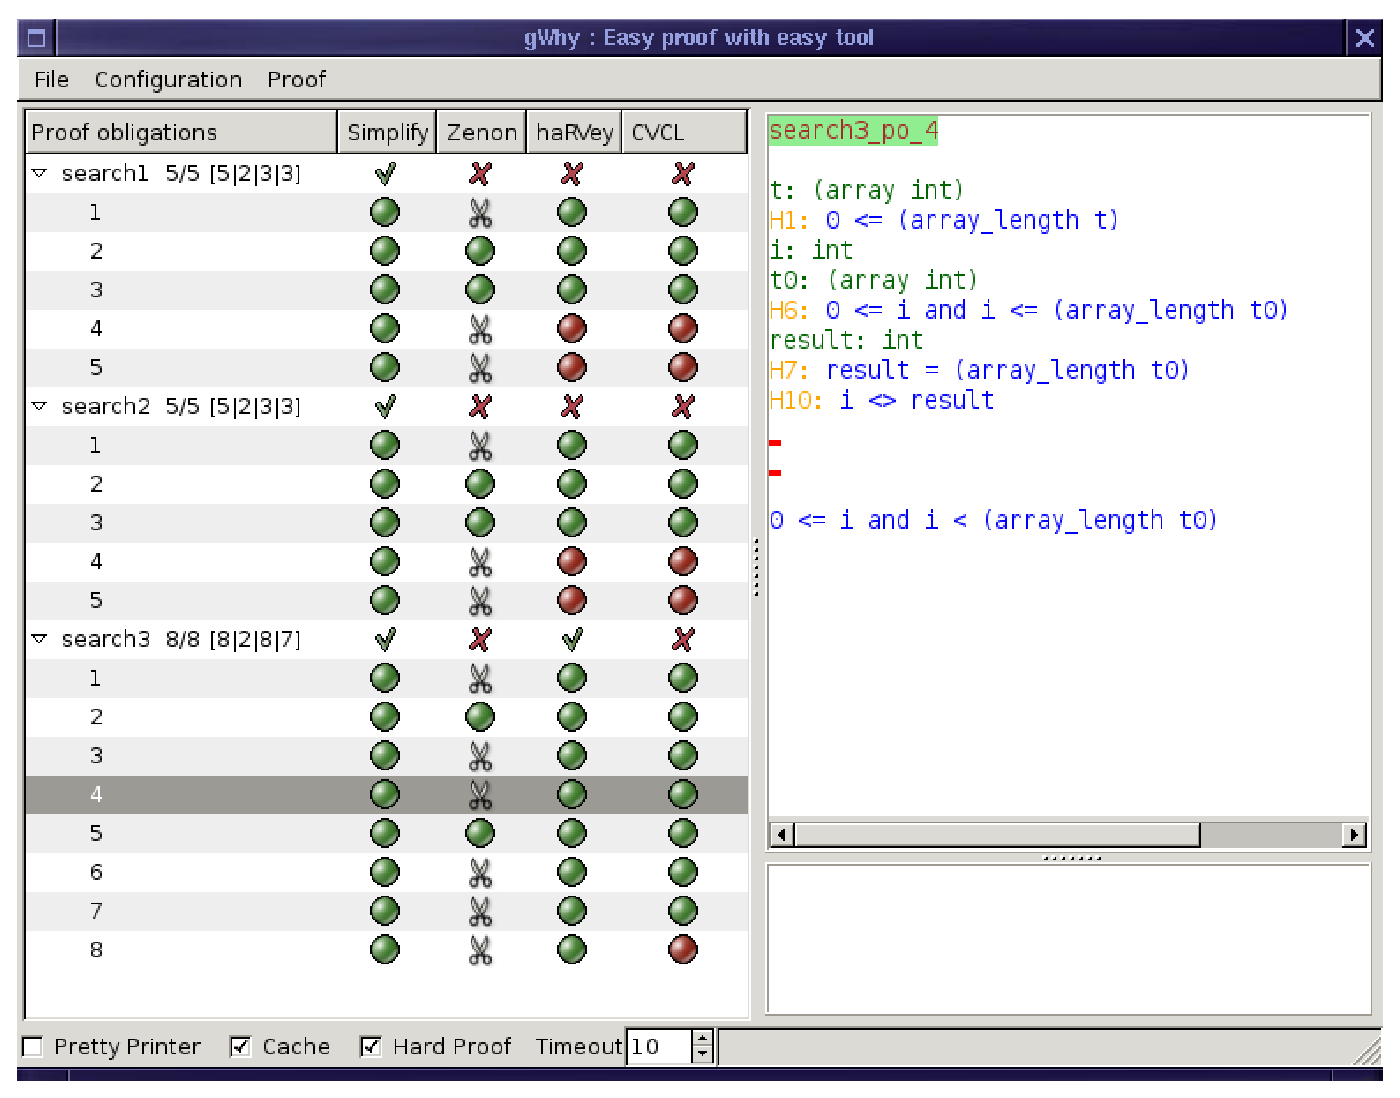
\includegraphics[width=0.8\textwidth]{gwhy-screenshot.eps}
  \caption{The \texttt{gwhy} graphical interface}
  \label{fig:gwhy}
\end{figure}

Note that you need the Unix \texttt{timeout} command to be installed
on your system before running \texttt{gwhy}.

\subsection{Calling decision procedures (\texttt{dp})}
\indextt{dp}

A small tool is provided to call the decision procedures (\simplify,
\harvey, \zenon\ and \cvclite) on files containing several goals, with
a timeout for each goal, and to display s short summary of the
results. Here is an example:
\begin{verbatim}
% dp -timeout 5 swap0_why.sx peano_why.sx
(. = valid * = invalid # = timeout/failure)
swap0_why.sx: ....... (7/0/0)
peano_why.sx: ............*...*..*.... (21/3/0)
total           :  31
valid           :  28 ( 90%)
invalid         :   3 ( 10%)
timeout/failure :   0 (  0%)
\end{verbatim}

Note: as for \texttt{gwhy}, you need the Unix \texttt{timeout} command
to be installed on your system to run \texttt{dp}.

\subsection{Why obfuscator (\texttt{why-obfuscator})}
\indextt{why-obfuscator}
A tool is provided to obfuscate some \why\ files. It is invoked as
follows:
\begin{center}
  \texttt{why-obfuscator} [\texttt{-o}
  \textit{file}]�~�[\texttt{-prefix} \textit{p}]
  files...
\end{center}
It produces a \why\ file equivalent to the set of \why\ files given as
arguments, where all identifiers are renamed and all comments
removed. The output is printed on the standard output unless
redirected with option \texttt{-o}. The identifiers are renamed as
\texttt{x1}, \texttt{x2}, ... unless a different name prefix is set
with option \texttt{-prefix}.

\subsection{Caml code generation (\texttt{why --ocaml})}
\label{ocamlcode}\index{Caml code generation}
In order to run your \why\ code, true \caml\ code can be
produced with option \texttt{--ocaml}: 
\begin{verbatim}
     why --ocaml foo.mlw
\end{verbatim}
When this option is selected, there is no generation of proof
obligations (\coq\ or \pvs\ files are not produced or updated).
The \caml\ code is written on standard output, unless redirected to
some file with option \texttt{--output} (see Section~\ref{usage}).

Programs' annotations can be inserted as comments in the \caml\ code,
with option \texttt{--ocaml-annot}. The default behavior is no
annotation. 

When the input file contains \texttt{parameter} declarations, the
\caml\ code generated is a functor, with these parameters as
arguments. For instance, the following input file
\begin{verbatim}
     parameter x : int ref
     let f (y:int) = x := !x + y
\end{verbatim}
is translated into the following piece of \caml\ code:
\begin{verbatim}
     module type Parameters = sig
       val x : int ref
     end

     module Make(P : Parameters) = struct
       open P
       let f = fun y (*:int*) -> x := !x + y
     end
\end{verbatim}
\texttt{external parameter} declarations are supposed to be realized by some
external \caml\ code. However, it is possible to make them arguments
of the functor too, with command line option \texttt{--ocaml-ext}.

\subsection{Why to HTML converter (\texttt{why2html})}
A tool to convert \why\ input files to HTML is provided. Its usage is
immediate:
\begin{verbatim}
     why2html [-t title] files...
\end{verbatim}
Each \why\ input file given on the command line, say \textit{foo.mlw},
is translated into a HTML file \textit{foo.mlw.html}. A title for the
HTML page can be specified using command line option \texttt{-t};
otherwise the original file name is used.


\section{Installation}
\label{install}\index{Installation}

To compile \why, you need \textsf{Objective Caml} to be
installed, in version at least 3.08. It can 
be fetched from \url{http://caml.inria.fr}.
Then 

\begin{enumerate}
\item Configure with \texttt{./configure}

  The directory for binaries defaults to \texttt{/usr/local/bin}; you
  can specify another directory with the \texttt{-{}-bindir}
  option. Similarly, you can change the directory for the library
  with \texttt{-{}-libdir} and for
  the man pages \texttt{-{}-mandir}.

\item Compile with \texttt{make}.

\item Install with \texttt{make install}.
\end{enumerate}


\section{Examples}
\label{examples}\index{Example}

Many examples are delivered with \why\ in the
subdirectory \texttt{examples/} of the distribution.
They are also available on the \why\ web site, at
\url{http://why.lri.fr/examples/}.


\section{Verifying C and Java programs}

C and \java\ programs can be verified using other tools in combination
with \why. C programs can be verified using \caduceus\ (see
\url{caduceus.lri.fr/}) and \java\ programs using \krakatoa\ (see
\url{krakatoa.lri.fr}). 


\chapter{Reference manual}
\label{refman}


\section{Command line}
\label{usage}\index{Option, of the command line}

\why\ is invoked as a batch compiler, given a list of input files:
\begin{center}
  \texttt{why} [\textit{options}] \textit{file}$_1$ $\cdots$ \textit{file}$_n$
\end{center}
If no file is given, then standard input is processed and output is
named with the prefix \texttt{out\_why} (and a suffix depending of the
selected prover).
The full list of command line options can be obtained with
\begin{verbatim}
  why --help
\end{verbatim}



\section{Syntax of input files}
\label{syntax}

\subsection{Lexical conventions}

Comments are opened with \texttt{(*}, closed
with \texttt{*)} and can be nested.

Identifiers are made of letters, digits,
the underscore character \texttt{\_} and the single quote \texttt{'},
starting with a letter. Additionally, they can be qualified by a
label (another identifier), using the \texttt{@} notation.

\begin{center}
\begin{tabular}{lrl}
  \nt{identifier}\indexnt{identifier}
    & $::=$ & \nt{letter} (\nt{letter} $|$ \te{0}..\te{9} $|$
              \te{\_} $|$ \te{'})\etoile
  \\[0.1em]
  \nt{letter}
    & $::=$ & \te{A}..\te{Z} $|$ \te{a}..\te{z}
  \\[0.1em]
  \nt{lab\_identifier}\indexnt{lab\_identifier}
    & $::=$ & \nt{identifier} [ \te{@} \nt{identifier} ]
\end{tabular}
\end{center}

Keywords are the following:
\begin{center}
{\tt\begin{tabular}{l@{\qquad}l@{\qquad}l@{\qquad}l@{\qquad}l}
        absurd &
	and &
        array &
	as &
	assert \\
	axiom &
	begin &
        bool &
	do &
	done \\
        else &
	end &
	exception &
	exists &
	external \\
        false &
	for &
	forall &
	fun &
	function \\
	goal &
	if &
	in &
	int &
	invariant \\
%	label &
	let &
	logic &
	not &
	of \\
	or &
	parameter &
	predicate &
	prop &
	raise \\
	raises &
	reads &
	real &
	rec &
	ref \\
	returns &
	then &
	true &
	try &
	type \\
	unit &
	variant &
	void &
	while &
	with \\
        writes &
\end{tabular}}
\end{center}

\subsection{Grammar}

\subsubsection{Logic}

Syntax for terms is given Figure~\ref{fig:terms}.
Arithmetical operations have usual precedences and are left associative.
The conditional construct \texttt{if $t_1$ then $t_2$ else $t_3$} can
also be written in prefix notation as \texttt{if\_then\_else($t_1$, $t_2$,
  $t_3$)}. 

Syntax for predicates is given Figure~\ref{fig:predicates}.
Precedences are the following (from strongest to weakest): \te{not}, 
\te{and}, \te{or}, implication, and \te{forall}. 
Implication, conjunction and disjunction are right associative.
Syntactic sugar: $t_1 ~ R_1 ~ t_2 ~ R_2 ~ t_3$ is equivalent to
$t_1 ~ R_1 ~ t_2 ~ \texttt{and} ~ t_2 ~ R_2 ~ t_3$ for any relations
$R_1$ and $R_2$. Example: \texttt{0 <= x < y} is \texttt{0 <= x and x
  < y}.

Syntax for logic declarations is given Figure~\ref{fig:ldecl}.

\begin{figure}[htbp]
\begin{center}
\hrulefill\\
\begin{tabular}{lrl}
  \nt{term}\indexnt{term}
    & $::=$ & \nt{constant} \\
      & $|$ & \nt{term} \nt{arith\_op} \nt{term} \\
      & $|$ & \te{-} \nt{term} \\
      & $|$ & \nt{lab\_identifier} \\
      & $|$ & \nt{identifier} \te{(} \nt{term}\plussep{\te{,}} \te{)} \\
      & $|$ & \nt{lab\_identifier} \te{[} \nt{term} \te{]} \\
      & $|$ & \te{if} \nt{term} \te{then} \nt{term} \te{else} \nt{term} \\
      & $|$ & \te{(} \nt{term} \te{)} \\
  \\[0.1em]

  \nt{constant}\indexnt{constant}
    & $::=$ & \nt{integer-constant} \\
      & $|$ & \nt{real-constant} \\
      & $|$ & \te{true} \\
      & $|$ & \te{false} \\
      & $|$ & \te{void} \\
  \\[0.1em]

  \nt{arith\_op}\indexnt{arith\_op}
    & $::=$ & \te{+} $|$ \te{-} $|$ \te{*} $|$ \te{/} $|$ \te{\%}
\end{tabular}\\
\hrulefill
\caption{Syntax of terms}
\label{fig:terms}
\end{center}            
\end{figure}

\begin{figure}[htbp]
\begin{center}
\hrulefill\\
\begin{tabular}{lrl}
  \nt{predicate}\indexnt{predicate}
    & $::=$ & \te{true} \\
      & $|$ & \te{false} \\
      & $|$ & \nt{identifier} \\
      & $|$ & \nt{identifier} \te{(} \nt{term}\plussep{\te{,}} \te{)} \\
      & $|$ & \nt{term} \nt{relation} \nt{term} 
              $[$ \nt{relation} \nt{term} $]$ \\
      & $|$ & \nt{predicate} \te{->} \nt{predicate} \\
      & $|$ & \nt{predicate} \te{<->} \nt{predicate} \\
      & $|$ & \nt{predicate} \te{or} \nt{predicate} \\
      & $|$ & \nt{predicate} \te{and} \nt{predicate} \\
      & $|$ & \te{not} \nt{predicate} \\
      & $|$ & \te{if} \nt{term} \te{then} \nt{predicate} 
              \te{else} \nt{predicate} \\
      & $|$ & \te{forall} \nt{identifier}\plussep{\te{,}}
              \te{:} \nt{primitive\_type}
              \te{.} \nt{predicate} \\
      & $|$ & \te{exists} \nt{identifier}\plussep{\te{,}}
              \te{:} \nt{primitive\_type}
              \te{.} \nt{predicate} \\
      & $|$ & \te{(} \nt{predicate} \te{)} \\
      & $|$ & (\nt{identifier} $|$ \nt{string}) \te{:} \nt{predicate} \\
  \\[0.1em]

  \nt{primitive\_type}\indexnt{primitive\_type}
    & $::=$ & \te{int} $|$ \te{bool} $|$ \te{real} $|$ 
              \te{unit} $|$ \nt{identifier} $|$ \te{'} \nt{identifier} \\
    & $|$ & \nt{primitive\_type} \nt{identifier} $|$ \te{(}
    \nt{primitive\_type}\etoilesep{\te{,}} \te{)} \nt{identifier} \\
  \\[0.1em]

  \nt{relation}\indexnt{relation}
    & $::=$ & \te{=} $|$ \te{<>} $|$ 
              \te{<} $|$ \te{<=} $|$ \te{>} $|$ \te{>=}
\end{tabular}\\
\hrulefill
\caption{Syntax of predicates}
\label{fig:predicates}
\end{center}            
\end{figure}

\begin{figure}[htbp]
\begin{center}
\hrulefill\\
\begin{tabular}{lrl}
  \nt{l\_declaration}
    & $::=$ & $[$ \te{external} $]$ \te{type} $[$ \nt{type\_parameters} $]$
              \nt{identifier} \\\indextt{type} \indextt{external}
      & $|$ & $[$ \te{external} $]$ \te{logic} \nt{identifier}\plussep{\te{,}}
              \te{:} \nt{logic\_type} \\\indextt{logic} \indextt{external}
      & $|$ & \te{function} \nt{identifier}
              \te{(} \nt{logic\_binder}\etoilesep{\te{,}}
              \te{)} \te{:} \nt{primitive\_type} \\
          & & \te{=} \nt{term} \\ \indextt{function}
      & $|$ & \te{predicate} \nt{identifier}
              \te{(} \nt{logic\_binder}\etoilesep{\te{,}}
              \te{)} \te{=} \nt{predicate} \\ \indextt{predicate}
      & $|$ & \te{axiom} \nt{identifier} \te{:} 
              \nt{predicate} \\\indextt{axiom}
      & $|$ & \te{goal} \nt{identifier} \te{:} 
              \nt{predicate} \\\indextt{goal}
   \\[0.1em]

  \nt{logic\_type}
    & $::=$ & \nt{logic\_arg\_type}\etoilesep{\te{,}} \te{->} \te{prop} 
              \\ \indextt{prop}
      & $|$ & \nt{logic\_arg\_type}\etoilesep{\te{,}} \te{->} 
              \nt{primitive\_type} \\ \indextt{logic}
   \\[0.1em]

  \nt{logic\_arg\_type}
    & $::=$ & \nt{primitive\_type} $|$ \nt{primitive\_type} \te{array} \\
   \\[0.1em]

   \nt{logic\_binder}
    & $::=$ & \nt{identifier} \te{:} \nt{primitive\_type} \\
   \\[0.1em]

   \nt{type\_parameters}
    & $::=$ & \te{'}\nt{identifier} $|$ 
              \te{(} (\te{'}\nt{identifier})\plussep{\te{,}} \te{)}
\end{tabular}\\
\hrulefill
\caption{Syntax of logic declarations}
\label{fig:ldecl}
\end{center}           
\end{figure}

\subsubsection{Programs}

Syntax of types is given Figure~\ref{fig:types}.
Syntax of annotated programs is given Figure~\ref{fig:caml}.
Syntax of input files is given Figure~\ref{fig:input}.

\begin{figure}[htbp]
\begin{center}
\hrulefill\\
\begin{tabular}{lrl}
  \nt{simple\_value\_type}\indexnt{simple\_value\_type}
    & $::=$ & \nt{primitive\_type} \\
      & $|$ & \nt{primitive\_type} \te{ref} \\
      & $|$ & \nt{primitive\_type} \te{array} \\
      & $|$ & \te{(} \nt{value\_type} \te{)} \\
  \\[0.1em]

  \nt{value\_type}\indexnt{value\_type}
    & $::=$ & \nt{simple\_value\_type} \\
      & $|$ & \nt{simple\_value\_type} \te{->} \nt{computation\_type} \\
      & $|$ & \nt{identifier} \te{:} \nt{simple\_value\_type} 
              \te{->} \nt{computation\_type} \\
  \\[0.1em]

  \nt{computation\_type}\indexnt{computation\_type}
    & $::=$ & \te{\{} $[$ \nt{precondition} $]$ \te{\}} \\
      &     & $[$ \te{returns} \nt{identifier} \te{:} $]$ \nt{value\_type}
              \nt{effects} \\
      &     & \te{\{} $[$ \nt{postcondition} $]$ \te{\}} \\
      & $|$ & \nt{value\_type} \\
  \\[0.1em]

  \nt{effects}
    & $::=$ & $[$ \te{reads} \nt{identifier}\etoilesep{\te{,}} $]$
              $[$ \te{writes}  \nt{identifier}\etoilesep{\te{,}}  $]$ 
              $[$ \te{raises}  \nt{identifier}\etoilesep{\te{,}}  $]$ \\
  \\[0.1em]

  \nt{precondition}\indexnt{precondition}
    & $::=$ & \nt{assertion} \\
  \\[0.1em]

  \nt{postcondition}\indexnt{postcondition}
    & $::=$ & \nt{assertion} \nt{exn\_condition}\etoile \\
  \\[0.1em]

  \nt{exn\_condition} 
    & $::=$ & \te{|} \nt{identifier} \te{=>} \nt{assertion} \\
  \\[0.1em]

  \nt{assertion} 
    & $::=$ & \nt{predicate} $[$ \te{as} \nt{identifier} $]$ \\
\end{tabular}\\
\hrulefill
\caption{Syntax of types}
\label{fig:types}
\end{center}            
\end{figure}

\begin{figure}[htbp]
\begin{center}
\hrulefill\\
\begin{tabular}{lrl}
  \nt{prog}\indexnt{prog}
    & $::=$ & \nt{constant} \\
      & $|$ & \nt{identifier} \\
      & $|$ & \te{!} \nt{identifier} \\
      & $|$ & \nt{identifier} \te{:=} \nt{prog} \\
      & $|$ & \nt{identifier} \te{[} \nt{prog} \te{]} \\
      & $|$ & \nt{identifier} \te{[} \nt{prog} \te{]} \te{:=} \nt{prog} \\
      & $|$ & \nt{prog} \nt{infix} \nt{prog} \\
      & $|$ & \nt{prefix} \nt{prog} \\
      & $|$ & \te{let} \nt{identifier} \te{=} \nt{prog} 
              \te{in} \nt{prog} \\
      & $|$ & \te{let} \nt{identifier} \te{=} \te{ref} 
              \nt{prog} \te{in} \nt{prog} \\
      & $|$ & \te{if} \nt{prog} \te{then} \nt{prog}
              $[$ \te{else} \nt{prog} $]$ \\
      & $|$ & \te{while} \nt{prog} \te{do}
              \nt{loop\_annot} \nt{prog} \te{done} \\
      & $|$ & \nt{prog} \te{;} \nt{prog} \\
      & $|$ & \nt{identifier} \te{:} \nt{prog} \\
      & $|$ & \te{assert} (\te{\{} \nt{assertion} \te{\}})\plus\
              \te{;} \nt{prog} \\
      & $|$ & \nt{prog} \te{\{}\ \nt{postcondition} \te{\}} \\
      & $|$ & \nt{prog} \te{\{\{}\ \nt{postcondition} \te{\}\}} \\
      & $|$ & \te{fun} \nt{binders} \te{->} \nt{prog} \\
      & $|$ & \te{let} \nt{identifier} \nt{binders} \te{=} \nt{prog} 
              \te{in}�\nt{prog} \\
      & $|$ & \te{let} \te{rec} \nt{recfun} $[$ \te{in} \nt{prog} $]$ \\
      & $|$ & \nt{prog} \nt{prog} \\
      & $|$ & \te{raise} \nt{identifier} $[$ \te{:} \nt{value\_type} $]$ \\
      & $|$ & \te{raise} \te{(} \nt{identifier} \nt{prog} \te{)}
              $[$ \te{:} \nt{value\_type} $]$ \\
      & $|$ & \te{try} \nt{prog} \te{with} 
              \nt{handler}\plussep{\te{|}} \te{end} \\
      & $|$ & \te{absurd} $[$ \te{:} \nt{value\_type} $]$ \\ \indextt{absurd}
      & $|$ & \te{(} \nt{prog} \te{)} \\
      & $|$ & \te{begin} \nt{prog} \te{end} \\
  \\[0.1em]

  \nt{infix}
    & $::=$ & \te{+} $|$ \te{-} $|$ \te{*} $|$ \te{/} $|$ \te{\%} $|$ 
              \te{=} $|$ \te{<>} $|$ 
              \te{<} $|$ \te{<=} $|$ \te{>} $|$ \te{>=} $|$
              \te{||} $|$ \te{\&\&} \\
  \nt{prefix}
    & $::=$ & \te{-} $|$ \te{not} \\
  \\[0.1em]

  \nt{binders}\indexnt{binders}
    & $::=$ & \te{(} \nt{identifier}\plussep{\te{,}} \te{:}
              \nt{value\_type} \te{)}\plus \\
  \\[0.1em]

  \nt{recfun}
    & $::=$ & \nt{identifier} \nt{binders} \te{:}
              value\_type \\
      &     & \te{\{} \te{variant} \nt{wf\_arg} \te{\}}
              \te{=} \nt{prog} \\
  \\[0.1em]

  \nt{loop\_annot}
    & $::=$ & \te{\{} \te{invariant} \nt{assertion} 
              \te{variant} \nt{wf\_arg} \te{\}} \\
  \\[0.1em]

  \nt{wf\_arg} 
    & $::=$ & \nt{term} $[$ \te{for} \nt{identifier} $]$ \\

  \\[0.1em]

  \nt{handler}\indexnt{handler}
    & $::=$ & \nt{identifier} \te{->} \nt{prog} \\
      & $|$ & \nt{identifier} \nt{identifier} \te{->} \nt{prog} \\
  
\end{tabular}\\
\hrulefill\caption{Syntax of annotated programs}
\label{fig:caml}
\end{center}
\end{figure}


\begin{figure}[htbp]
\begin{center}
\hrulefill\\
\begin{tabular}{lrl}
  \nt{file}
    & $::=$ & \nt{declaration}\etoile\ \\
  \\[0.1em]

  \nt{declaration}
    & $::=$ & \te{let} \nt{identifier} $[$ \nt{binders} $]$ \te{=} \nt{prog} \\
      & $|$ & \te{let} \te{rec} \nt{recfun} \\
      & $|$ & $[$ \te{external} $]$ 
              \te{parameter} \nt{identifier}\plussep{\te{,}}
              \te{:} \nt{value\_type} \\ \indextt{parameter}\indextt{external}
      & $|$ & \te{exception} \nt{identifier} 
              $[$ \te{of} \nt{primitive\_type} $]$ \\ \indextt{exception}
      & $|$ & \nt{l\_declaration}
\end{tabular}\\
\hrulefill
\caption{Syntax of input files}
\label{fig:input}
\end{center}           
\end{figure}

\section{Semantics}

\subsection{Logic}

The abstract syntax for types ($\tau$), terms ($t$) and predicates
($P$) is given by the following grammars:
\begin{displaymath}
  \begin{array}{rrl}
    \tau & ~::=~ & \alpha ~|~ (\tau,\dots,\tau)~s \\
    t & ~::=~ & x ~|~ f(t,\dots,t) \\
    P & ~::=~ & p(t,\dots,t) \\ 
      &    |~~ & \top ~|~ \bot ~|~ P \land P ~|~ P \lor P
                 ~|~ \lnot P ~|~ P\Rightarrow P \\
      &    |~~ & \forall x:\tau.\,P ~|~ \exists x:\tau.\,P
  \end{array}
\end{displaymath}
A theory $\Sigma$ is a finite list of declarations $\delta$ where
\begin{displaymath}
  \begin{array}{rrl}
  \delta & ~::=~ & 
      \texttt{type}~\vec{\alpha}~s ~|~ x:\tau ~|~
      \mathtt{logic}~f:\forall\vec{\alpha}.\,\tau,\dots,\tau\rightarrow\tau \\
         &    |~~ &   
      \mathtt{logic}~p:\forall\vec{\alpha}.\,\tau,\dots,\tau\rightarrow\mathtt{prop} ~|~ 
      \texttt{axiom}~\forall\vec{\alpha}.\,P ~|~
      \texttt{goal}~\forall\vec{\alpha}.\,P \\
  \end{array} 
\end{displaymath}

\subsubsection{Typing}

\newcommand{\kw}[1]{\ensuremath{\mathsf{#1}}}
\newcommand{\wf}[1]{#1~\kw{wf}}
\newcommand{\Subst}[2]{\ensuremath{\mathsf{Subst}(#1,#2)}}

Well-formed types ($\Sigma\vdash\wf{\tau}$):
% types wf
\begin{displaymath}
  \frac{}{\Sigma\vdash\wf{\alpha}}(\mathsf{Ty}_1)
  \qquad
  \frac{\mathtt{type}~(\alpha_1,\dots,\alpha_n)~s\in\Sigma
        \quad
        \forall i,\,\Sigma\vdash\wf{\tau_i}}
       {\Sigma\vdash\wf{(\tau_1,\dots,\tau_n)~s}}(\mathsf{Ty}_2)
\end{displaymath}
Well-typed terms ($\Sigma\vdash t:\tau$):
\begin{displaymath}
  \frac{x:\tau\in\Sigma}{\Sigma\vdash x:\tau}(\mathsf{T}_1)
  \qquad
  \frac{
    \begin{array}{c}
      \texttt{logic}~f:\forall\vec{\alpha}.\,\tau_1,\dots,\tau_n\rightarrow\tau\in\Sigma \\[0.2em]
      \Subst{\sigma}{\Sigma} \quad
       \forall i,\, \Sigma\vdash t_i:\sigma(\tau_i) \\
    \end{array}}
       {\Sigma\vdash f(t_1,\dots,t_n):\sigma(\tau)}(\mathsf{T}_2)
\end{displaymath}
\begin{description}
\item[~~~]
  where $\sigma$ is a mapping from type variables to types, naturally
  extended to types with $\sigma((\tau_1,\dots,\tau_n)~s) =
  (\sigma(\tau_1),\dots,\sigma(\tau_n))~s$. 
  We write $\Subst{\sigma}{\Sigma}$ whenever
  $\Sigma\vdash\wf{\sigma(\alpha)}$ holds for any type variable $\alpha$.
\end{description}
Well-typed predicates ($\Sigma\vdash\wf{P}$):
\begin{displaymath}
 \frac{
    \begin{array}{c}
      \texttt{logic}~p:\forall\vec{\alpha}.\,\tau_1,\dots,\tau_n\rightarrow\mathtt{prop}\in\Sigma \quad
        \Subst{\sigma}{\Sigma} \quad
        \forall i,\,\Sigma\vdash t_i:\sigma(\tau_i) \\
    \end{array}}
       {\Sigma\vdash\wf{p(t_1,\dots,t_n)}}(\mathsf{P}_1)
\end{displaymath}
\begin{displaymath}
  \frac{}
       {\Sigma\vdash\wf{\top}}(\mathsf{P}_2)
  \qquad
  \frac{}
       {\Sigma\vdash\wf{\bot}}(\mathsf{P}_3)
  \qquad
  \frac{\Sigma\vdash\wf{P_1} \quad \Sigma\vdash\wf{P_2}}
       {\Sigma\vdash\wf{P_1\land P_2}}(\mathsf{P}_4)
\end{displaymath}
\begin{displaymath}
  \frac{\Sigma\vdash\wf{P_1} \quad \Sigma\vdash\wf{P_2}}
       {\Sigma\vdash\wf{P_1\lor P_2}}(\mathsf{P}_5)
  \qquad
  \frac{\Sigma\vdash\wf{P}}
       {\Sigma\vdash\wf{\lnot P}}(\mathsf{P}_6)
\end{displaymath}
\begin{displaymath}
  \frac{\Sigma\vdash\wf{P_1} \quad \Sigma\vdash\wf{P_2}}
       {\Sigma\vdash\wf{P_1\Rightarrow P_2}}(\mathsf{P}_7)
\end{displaymath}
\begin{displaymath}
  \frac{\Sigma,x:\tau\vdash\wf{P}}
       {\Sigma\vdash\wf{\forall x:\tau.\,P}}(\mathsf{P}_8)
  \qquad
  \frac{\Sigma,x:\tau\vdash\wf{P}}
       {\Sigma\vdash\wf{\exists x:\tau.\,P}}(\mathsf{P}_8)
\end{displaymath}
Well-formed theories ($\vdash\wf{\Sigma}$):
\begin{displaymath}
  \frac{}{\vdash\wf{\emptyset}}(\textsf{Th}_1)
  \qquad
  \frac{\texttt{type}~s\not\in\Sigma}
       {\vdash\wf{\Sigma,\texttt{type}~(\alpha_1,\dots,\alpha_n)~s}}(\textsf{Th}_2)
  \qquad
  \frac{x\not\in\Sigma \quad \Sigma\vdash\wf{\tau}}
       {\vdash\wf{\Sigma,x:\tau}}(\textsf{Th}_3)
\end{displaymath}
\begin{displaymath}
  \frac{\texttt{logic}~f\not\in\Sigma \quad
        \forall i,\, \Sigma\vdash\wf{\tau_i}}
       {\vdash\wf{\Sigma,\mathtt{logic}~f:\forall\vec{\alpha}.\,\tau_1,\dots,\tau_n\rightarrow\tau_{n+1}}}(\textsf{Th}_4)
\end{displaymath}
\begin{displaymath}
  \frac{\texttt{logic}~p\not\in\Sigma \quad
        \forall i,\, \Sigma\vdash\wf{\tau_i}}
       {\vdash\wf{\Sigma,\mathtt{logic}~p:\forall\vec{\alpha}.\,\tau_1,\dots,\tau_n\rightarrow\mathtt{prop}}}(\textsf{Th}_5)
\end{displaymath}
\begin{displaymath}
  \frac{\Sigma\vdash\wf{P}}
       {\vdash\wf{\Sigma,\texttt{axiom}~\forall\vec{\alpha}.\,P}}(\textsf{Th}_6)  \qquad
  \frac{\Sigma\vdash\wf{P}}
       {\vdash\wf{\Sigma,\texttt{goal}~\forall\vec{\alpha}.\,P}}(\textsf{Th}_6)  
\end{displaymath}
Well-formed definitions of functions and predicates:
\begin{displaymath}
  \frac{\Sigma\vdash\wf{\tau_i} \quad
        \Sigma,x_1:\tau_1,\dots,x_n:\tau_n\vdash t:\tau}
       {\Sigma\vdash\wf{\mathtt{function}~f(x_1:\tau_1,\dots,x_n:\tau_n) : \tau = t}}(\textsf{Th}_7)
\end{displaymath}
\begin{displaymath}
  \frac{\Sigma\vdash\wf{\tau_i} \quad
        \Sigma,x_1:\tau_1,\dots,x_n:\tau_n\vdash\wf{P}}
       {\Sigma\vdash\wf{\mathtt{predicate}~p(x_1:\tau_1,\dots,x_n:\tau_n) = P}}(\textsf{Th}_8)
\end{displaymath}
Then, as far as typing and validity in concerned, the function $f$
(resp. the predicate $p$) is added to $\Sigma$ as 
$\mathtt{logic}~f:\tau_1,\dots,\tau_n\rightarrow\tau$
(resp. $\mathtt{logic}~p:\tau_1,\dots,\tau_n\rightarrow\mathtt{prop}$).

\subsubsection{Validity}

Validity is defined as a set of natural deduction rules
($\Sigma\models P$). For the sake of clarity, 
we write $\Sigma,P$ for $\Sigma,\texttt{axiom}~P$ in the following.
A substitution $\sigma$ over from type variables to types in extended
to terms and predicates in the obvious way. We write $P[t/x]$ for the
substitution of all the occurrences of a free variable $x$ in $P$ by a
term $t$. 
\begin{displaymath}
  \frac{\texttt{axiom}~\forall\vec{\alpha}.\,P\in\Sigma \quad
        \Subst{\sigma}{\Sigma}}
       {\Sigma\models\sigma(P)}(\mathsf{Ax})
  \qquad
  \frac{\Sigma\models Q \quad 
        \Sigma,Q\models P}
       {\Sigma\models P}(\mathsf{Cut})
\end{displaymath}
\begin{displaymath}
  \frac{}{\Sigma\models\top}(\mathsf{True})
  \qquad
  \frac{\Sigma\models\bot \quad \Sigma\vdash\wf{P}}
       {\Sigma\models P}(\mathsf{False})
  \qquad
  \frac{\Sigma\vdash\wf{P}}{\Sigma\models P\lor\lnot P}(\mathsf{EM})
\end{displaymath}
% and
\begin{displaymath}
  \frac{\Sigma\models P \quad \Sigma\models Q}
       {\Sigma\models P\land Q}(\mathsf{And}_1)
  \qquad
  \frac{\Sigma\models P\land Q}
       {\Sigma\models P}(\mathsf{And}_2)
  \qquad
  \frac{\Sigma\models P\land Q}
       {\Sigma\models Q}(\mathsf{And}_3)
\end{displaymath}
% or
\begin{displaymath}
  \frac{\Sigma\models P \quad \Sigma\vdash\wf{Q}}
       {\Sigma\models P\lor Q}(\mathsf{Or}_1)
  \qquad
  \frac{\Sigma\models Q \quad \Sigma\vdash\wf{P}}
       {\Sigma\models P\lor Q}(\mathsf{Or}_2)
\end{displaymath}
\begin{displaymath}
  \frac{\Sigma\models P\lor Q \quad
        \Sigma,P\models R \quad \Sigma,Q\models R}
       {\Sigma\models R}(\mathsf{Or}_3)
\end{displaymath}
% not
\begin{displaymath}
  \frac{\Sigma\vdash\wf{P} \quad \Sigma,P\models\bot}
       {\Sigma\models\lnot P}(\mathsf{Not}_1)
  \qquad
  \frac{\Sigma\models P \quad \Sigma\models\lnot P}
       {\Sigma\models\bot}(\mathsf{Not}_2)
\end{displaymath}
% implies
\begin{displaymath}
  \frac{\Sigma\vdash\wf{P} \quad \Sigma,P\models Q}
       {\Sigma\models P\Rightarrow Q}(\mathsf{Imp}_1)
  \qquad
  \frac{\Sigma\models P\Rightarrow Q \quad \Sigma\models P}
       {\Sigma\models Q}(\mathsf{Imp}_2)
\end{displaymath}
% forall
\begin{displaymath}
  \frac{x\not\in\Sigma \quad
        \Sigma\vdash\wf{\tau} \quad 
        \Sigma,x:\tau\models P}
       {\Sigma\models\forall x:\tau.\,P}(\mathsf{Forall}_1)
\end{displaymath}
\begin{displaymath}
  \frac{\Sigma\models\forall x:\tau.\,P \quad
        \Sigma\vdash t:\tau}
       {\Sigma\models P[t/x]}(\mathsf{Forall}_2)
\end{displaymath}
% exists
\begin{displaymath}
  \frac{%\Sigma\vdash\wf{\tau} \quad INUTILE CAR CONSEQUENCE
        \Sigma\vdash t:\tau \quad
        x\not\in\Sigma \quad
        \Sigma\models P[t/x]}
       {\Sigma\models\exists x:\tau.\,P}(\mathsf{Exists}_1)
\end{displaymath}
\begin{displaymath}
  \frac{\Sigma\models\exists x:\tau.\,P \quad
        x\not\in\Sigma \quad
        \Sigma,x:\tau,P\models Q}
       {\Sigma\models Q}(\mathsf{Exists}_2)
\end{displaymath}
Deduction rules for equality: 
\begin{displaymath}
  \frac{\Sigma\vdash t:\tau}
       {\Sigma\models t=t}(\mathsf{Eq}_1)
  \qquad
  \frac{\Sigma\models x=y \quad
        \Sigma,z:\tau\vdash\wf{P} \quad 
        \Sigma\models P[x/z]}
       {\Sigma\models P[y/z]}(\mathsf{Eq}_2)
\end{displaymath}
Arithmetic:
An arithmetic proposition $P$ is a proposition built from 
variables of type \textit{int}, integers constants,
the functions symbols \textit{add\_int} and \textit{sub\_int}, the predicates
\textit{lt\_int, le\_int, gt\_int, ge\_int} and the equality.
If $x_1,\dots,x_n$ are the free variables of $P$,
we write $x_1,\dots,x_n\models_A P$ whenever $P$ is valid in
Presburger arithmetic (which is decidable).
Then we have the following deduction rule for arithmetic:
\begin{displaymath}
  \frac{x_1,\dots,x_n\models_A P}
       {\Sigma\models\forall x_1:\mathit{int}.\,\dots\forall
         x_n:\mathit{int}.\, P}(\mathsf{Arith})
\end{displaymath}


\subsection{Programs}

\subsubsection{Typing}

\subsubsection{Weakest preconditions}


\section{Prelude}
\label{prelude}\index{Prelude}

Apart from the type names \texttt{unit}, \texttt{bool}, \texttt{int},
\texttt{real}, and the type constructor \texttt{ref}, nothing is
built-in in the \why\ tool. But a prelude 
file is read before considering the files given on the command
line. The prelude file lies in \url{/usr/local/lib/why/prelude.why}
(if your library path was not set differently).
The interpretation of this prelude is prover-dependent. 
It is possible not to load the prelude using the command-line option
\texttt{--no-prelude}.
The remaining of this section describes the contents of the prelude.

{\small
\verbatiminput{../lib/why/prelude.why}
}

\section{Provers specificities}

\subsection{Coq}
\label{lib:coq}\index{Coq library}

Several \coq\ modules are delivered with \why. If installation is
properly done, they should be found in subdirectory \texttt{user-contrib}
of the \coq\ standard library (usually \texttt{/usr/lib/coq}
unless some other path was specified when installing \coq). 

% \coq\ files generated by \why\ usually start with \texttt{Require Why}
% (unless specified otherwise using command line option
% \texttt{--coq-preamble}). For this module to be found by \coq, the
% \coq\ load path must be set accordingly, either using the \coq\ command
% line option \texttt{-I} or the \coq\ command \texttt{Add LoadPath} (to
% be put in a \texttt{.coqrc} file for instance).

\paragraph{Types.} 
Types are mapped as follows:
\begin{center}
  \begin{tabular}{|l|l|}
    \hline
    \why & \coq \\
    \hline
    \texttt{unit} & \texttt{unit} \\
    \hline
    \texttt{bool} & \texttt{bool} \\
    \hline
    \texttt{int} & \texttt{Z} \\
    \hline
    \texttt{real} & \texttt{R} \\
    \hline
    $\tau$ \texttt{array} & \texttt{(array $\tau$)},
                            from module \texttt{WhyArrays} \\
    \hline
  \end{tabular}
\end{center}

\paragraph{Arrays.} 
Arrays are introduced in module \texttt{WhyArrays}. 
Some tactics are provided to help the user simplifying array expressions
in proof obligations:
\begin{description}
\item[\texttt{WhyArrays}] : repeatedly simplifies
  \texttt{access}/\texttt{update}using combinations and
  \texttt{array\_length} expressions
\item[\texttt{AccessSame}] : rewrites
  $\texttt{access}~(\mathtt{update}~t~i~v)~i$  into $v$,
  simplifies with \texttt{WhyArrays} and attempts \texttt{omega} on
  every subgoal
\item[\texttt{AccessOther}] : rewrites 
    $\texttt{access}~(\mathtt{update}~t~i~v)~j$  into $\mathtt{access}~t~j$,
  simplifies with \texttt{WhyArrays} and attempts \texttt{omega} on
  every subgoal
\item[\texttt{ArraySubst} $t$] : similar to \texttt{subst $t$}, with
  additional simplifications
\end{description}

\subsection{PVS}
\label{lib:pvs}\index{PVS library}

\paragraph{Types.} 
Types are mapped as follows:
\begin{center}
  \begin{tabular}{|l|l|}
    \hline
    \why & \coq \\
    \hline
    \texttt{unit} & \texttt{unit}, from theory \texttt{why} \\
    \hline
    \texttt{bool} & \texttt{bool} \\
    \hline
    \texttt{int} & \texttt{int} \\
    \hline
    \texttt{real} & \texttt{real} \\
    \hline
    $\tau$ \texttt{array} & \texttt{warray[$\tau$]},
                            from theory \texttt{why} \\
    \hline
  \end{tabular}
\end{center}

\paragraph{Arrays.} An array whose elements are of type \texttt{T} is a
\pvs\ value of type \texttt{warray[T]}. This type is defined in the
theory \texttt{why\_arrays}, as
a pair of an integer, the array length, and a function mapping
indices to elements :
\begin{verbatim}
     warray: TYPE = [ n:int, [ below(n) -> T ] ]
\end{verbatim}
Two other theories, \texttt{why\_int\_array\_pred} and
\texttt{why\_array\_pred}, introduce the various predicates over
arrays presented in Section~\ref{prelude}.


\nocite{*}
\bibliographystyle{plain}
\bibliography{./biblio}


\newpage
\addcontentsline{toc}{chapter}{Index}
\printindex

\end{document}
